\section{Python scripts}
\label{sec:python}

Basic functionality of the Fortran-based software describen in Sec.~\ref{Sec.FortranProgram} was compiled as a Python library (module). The installation is performed similar to \ref{Sec:Install}, with additional key for configure script:
\begin{verbatim}
    ./configure --enable-python
\end{verbatim}
After successful installation created library (which can be used as Python module) is available in {\tt ./bin/averager.so }

The code, which implement Fortran to Python interface is in file:  {\tt ./source/average\_py.f90} (written in Fortran90).

Several scripts written in python are provided to support Python-based averaging.

\begin{itemize}
\item {\tt DatasetGen.py}: Script to generate random dataset, which can be used for testing averagerr
\item {\tt DataReader.py}: Module to parse data-files and read data in Python variables
\item {\tt test.py}: Script which shows an example of using Python-based averagerr
\end{itemize}

The {\tt test.py} file demonstrates the work of data reader and Python=-based averager. Also it contains a plotting part.

\subsubsection{Data reader}

Data reader module {\tt DataReader} read the data from all {\tt .csv} files in current directory. The nodule consists of one a function {\tt paverager(bins,data,error)}, where:

\begin{itemize}
\item {\tt bins}: names of bin columns ('bin1,bin2,...'). If the input string is empty all columns with substring 'bin' are considered as bins. 
\item {\tt data}: name of measurement column (input as 'data1'). If the input string is empty column 'data' is considered as measurement.
\item {\tt error}: names of uncertainty columns. Columns with substring 'stat' are considered as bin-to-bin uncorrelated. At least one column should be bin-to-bin uncorrelated for statistical uncertainty ('error1:M,error2,stat,...'). Different uncertainties should have different names. If the input string is empty all column with substring 'error' are considered as bin-to-bin correlated uncertainty, all columns with substring 'stat' are considered as bin-to-bin uncorrelated uncertainty.
\end{itemize}

The function return 3 lists: measurements, their systematic and statistical uncertainties. All considered bin-to-bin uncorrelated uncertainties are summed quadratically and considered as statistical uncertainty.

Example of usage:
\begin{verbatim}
mes,stat,syst=DataReader.paverager('','','')
\end{verbatim}


The format of the input data-file is following:
\begin{verbatim}
bin1,bin2,data,stat,error00000,error00001,error00002,error00004
0,1,14.01,0.261,1.499,1.43,-1.293,1.334
5,1,37.7,0.552,3.829,3.461,-2.908,4.197
6,1,1.84,0.048,0.167,0.167,-0.15,0.157
7,1,69.75,1.918,7.331,7.194,-5.481,6.44
8,1,6.44,0.169,0.502,0.659,-0.665,0.514
9,1,58.61,1.456,6.055,7.045,-5.182,6.405
10,1,3.03,0.041,0.293,0.275,-0.217,0.281
12,1,6.46,0.089,0.63,0.649,-0.534,0.611
13,1,23.79,0.345,2.44,2.279,-2.026,2.233
14,1,11.67,0.303,1.293,1.293,-0.839,0.582
17,1,9.64,0.253,1.12,0.75,-1.042,0.974
\end{verbatim}
Here header contains the name of the columns (separated by ``,'').

Lists of systematic-names {\tt snames} and file-names {\tt fnames} can be extracted using corresponding global variables: {\tt oerror} and {\tt fnames}.

\begin{verbatim}
snames=DataReader.oerror
fnames=DataReader.fnames
\end{verbatim}

\subsubsection{Generation of random dataset}

Parameters of the data-set generator are given in the beginning of the script in following variables:
\begin{itemize}
\item {\tt nData} (integer): Number of data points
\item {\tt nMes} (list of 3 integers): Total number of measurements, minimal and maximal number of measurements per data point (have to be smaller as total number of measurements). In case if minimal, maximal and total are the same, each data point will have the same number of measurements.
\item {\tt nSyst} (list of 3 integers): Total number of systematic uncertainties, minimal and maximal number of correlated systematic uncertainties per measurement (have to be smaller as total number of systematic uncertainties). In case if minimal, maximal and total are the same, each measurement will have the same systematic uncertainties.
\item {\tt vStat} (list of 2 floats): Minumal and maximal relative statistical uncertainty
\item {\tt vSyst} (list of 2 floats): Minumal and maximal relative systematic uncertainty
\end{itemize}

The output of the generator is stored in text files (Each measurement is in separate file):
\begin{itemize}
\item {\tt test0.dat, test1.dat, ...} -- suitable for the Fortran-based averager.
\item {\tt test0.csv, test1.csv, ...} -- suitable for the Python-based averager.
\end{itemize}

\subsection{Python-based averager}
\label{Sec:PythonUsing}

Pythin-based averager can be imported as module {\tt averager}. The function, which performs the averaging have 3 input and 3 output parameters:
\begin{verbatim}
ave,statOut,systOut = averager.averager(mes,stat,syst)
\end{verbatim}
where:

\begin{itemize}
\item {\tt mes} -- measurements
\item {\tt stat,syst} -- statistical and systematic uncertainties of the measurements.
\item {\tt ave} -- average values
\item {\tt statOut,systOut} -- statistical and systematic uncertainties of the average values.
\end{itemize}
Input parameters are prepared by {\tt DataReader}.

Default parameters of the averager can be modified by changing global variables of the {\tt averager}. In this case averager have to be initialized before these changes. Otherwise all parameters will be overwritten by their default values.

\begin{verbatim}
#initialization
averager.avin.initvariables()

averager.avin.indebug = 0
averager.avin.inwriteoriginal = .false.
averager.avin.inwritesystextable = .false.
averager.avin.inpostrotatesyst = .false.

averager.avin.setoutputprefix('Ave')
averager.avin.setoutputfolder('../output')
averager.avin.setsnames(snames)


averager.avin.initeration = 10
averager.avin.inrescalestatsep = .false.
averager.avin.inborrectbtatbias = .false.
averager.avin.infixstat = .false.
\end{verbatim}
Parameters given here are default parameters. All variable have the same meaning as for the Fortran-base program (see Sec.~\ref{Sec:Steerign}). Output mode is always orthogonal.

Names of the systematic uncertainties are given by the list of names {\tt snames}. If names are not given all systematics are considered as symmetric, multiplicative.

Additional output information of the averaging is available with following variables

\begin{itemize}
\item {\tt averager.avout.pulldata} -- pulls of data
\item {\tt averager.avout.pullsyst} -- pulls of systematic uncertainties
\item {\tt averager.avout.shiftsyst} -- shift of systematic uncertainties
\item {\tt averager.avout.squeezesyst} -- reduction of the systematic uncertainties
\item {\tt averager.avout.chi2} -- $\chi^2$
\item {\tt averager.avout.ndof} -- number degrees of freedom
\end{itemize}

\subsection{Python-based plotting}
\label{Sec:PythonPlotting}

Some examples of plotting functionality is shown in the {\tt test.py}. Script plots the averaged data and pull of systematic uncertainties. Results are stored in pdf files. An example of output plot is shown below.

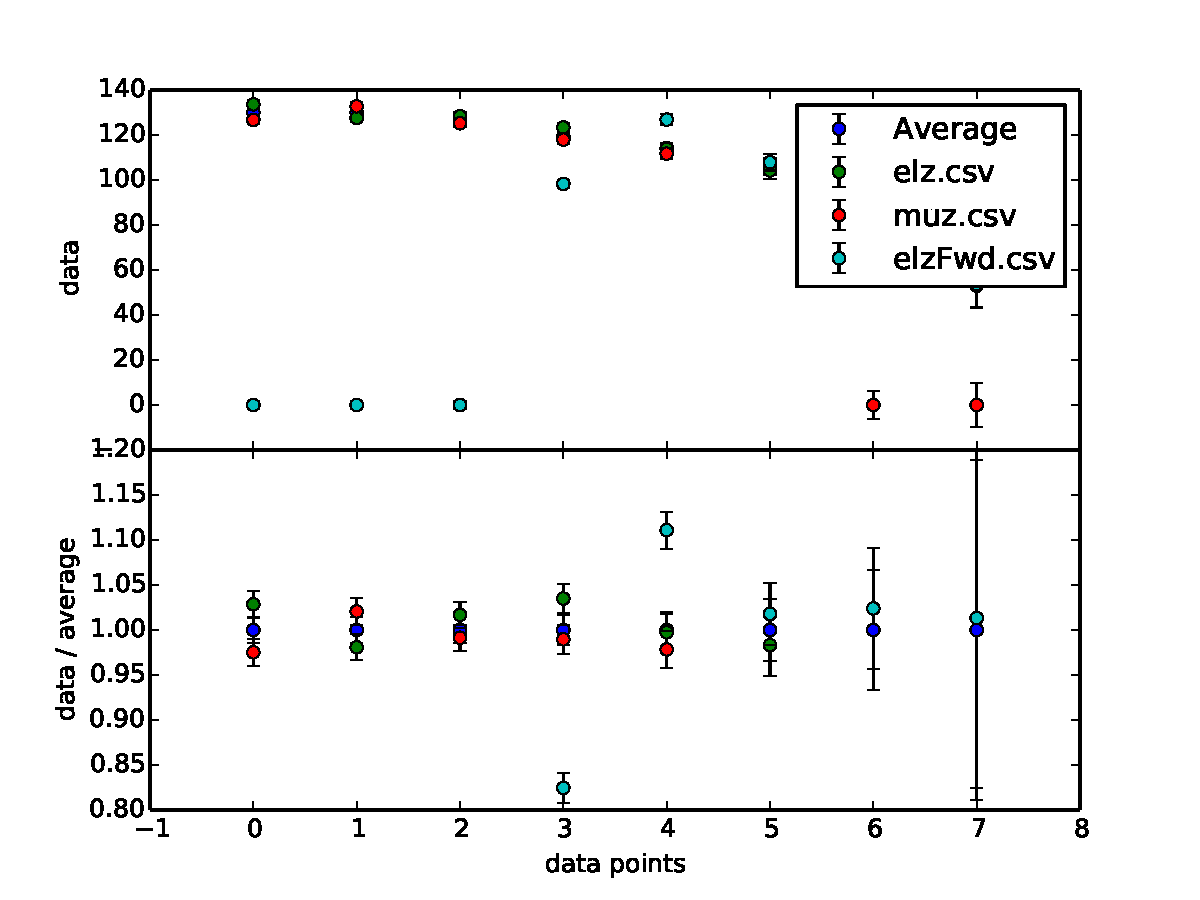
\includegraphics[width=0.49\linewidth]{figures/AvData.pdf}
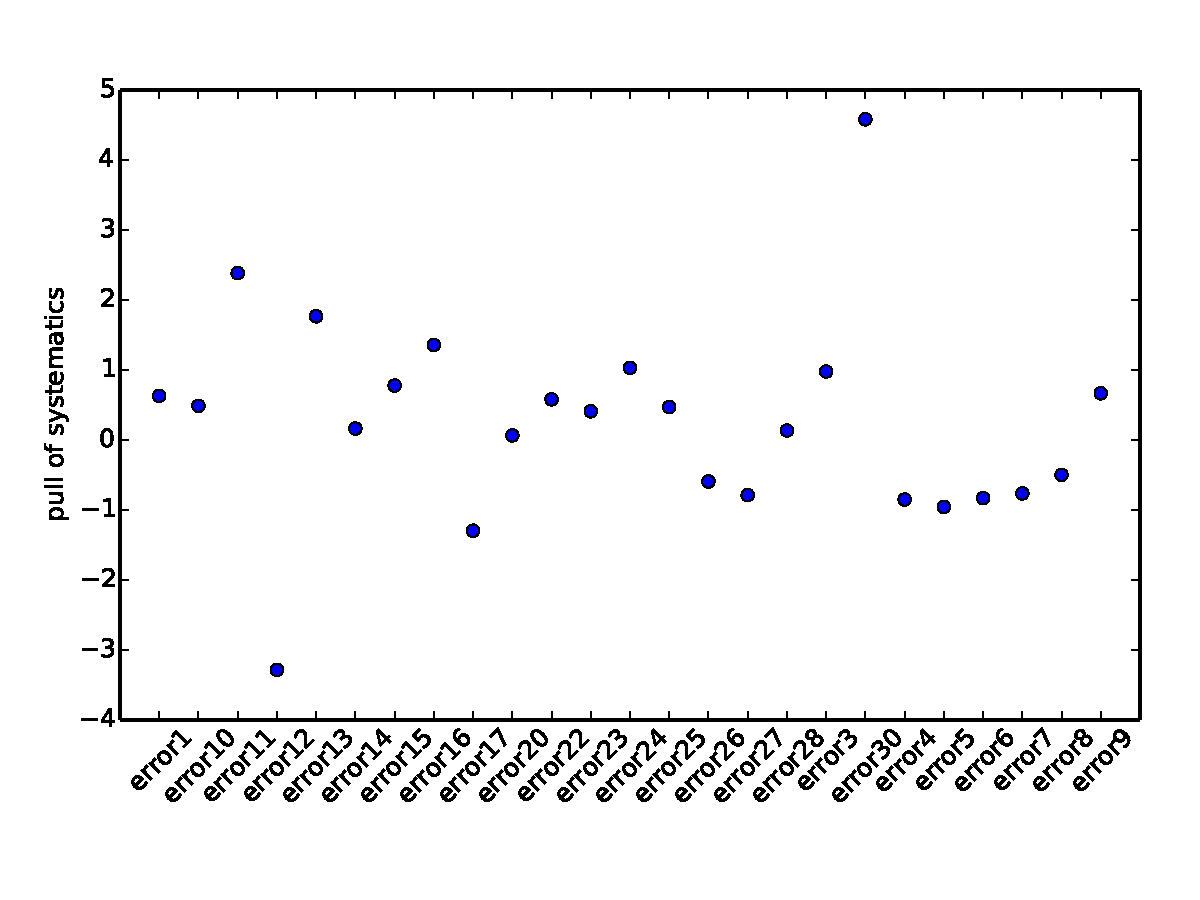
\includegraphics[width=0.49\linewidth]{figures/AvPull.pdf}

Additionally a script {\tt plot.py} plot histograms of data pulls and systematic pulls using text files as input. Therefore this script can be used also to visualise output of the fortran-base averager. Using of the script is following: 

\begin{verbatim}
./plot.py output
\end{verbatim}

where {\tt output} is the path to the output folder of the averager. This script reads files: {\tt sys.txt, tab.dat, chi2map.dat} and save plots as pdf files.
